% Chapter Template

\chapter{Implémentation} % Main chapter title

\label{Chapter3} % Change X to a consecutive number; for referencing this chapter elsewhere, use \ref{ChapterX}

\lhead{Chapitre 3. \emph{Implémentation}} % Change X to a consecutive number; this is for the header on each page - perhaps a shortened title

%----------------------------------------------------------------------------------------
%	SECTION 1
%----------------------------------------------------------------------------------------

\section{Diagrammes de packages et de classes rétro-générés}

\subsection{Architecture générale}
\begin{figure}[H]
	\centering
		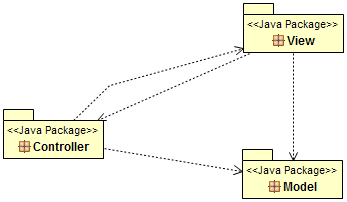
\includegraphics{Figures/retro_archi}
		\rule{35em}{0.5pt}
	\caption[Vue générale de l'application]{Vue générale de l'application}
\end{figure}

\subsection{Package model}
\subsubsection{Diagramme de classes rétro-générés}
\begin{figure}[H]
	\centering
		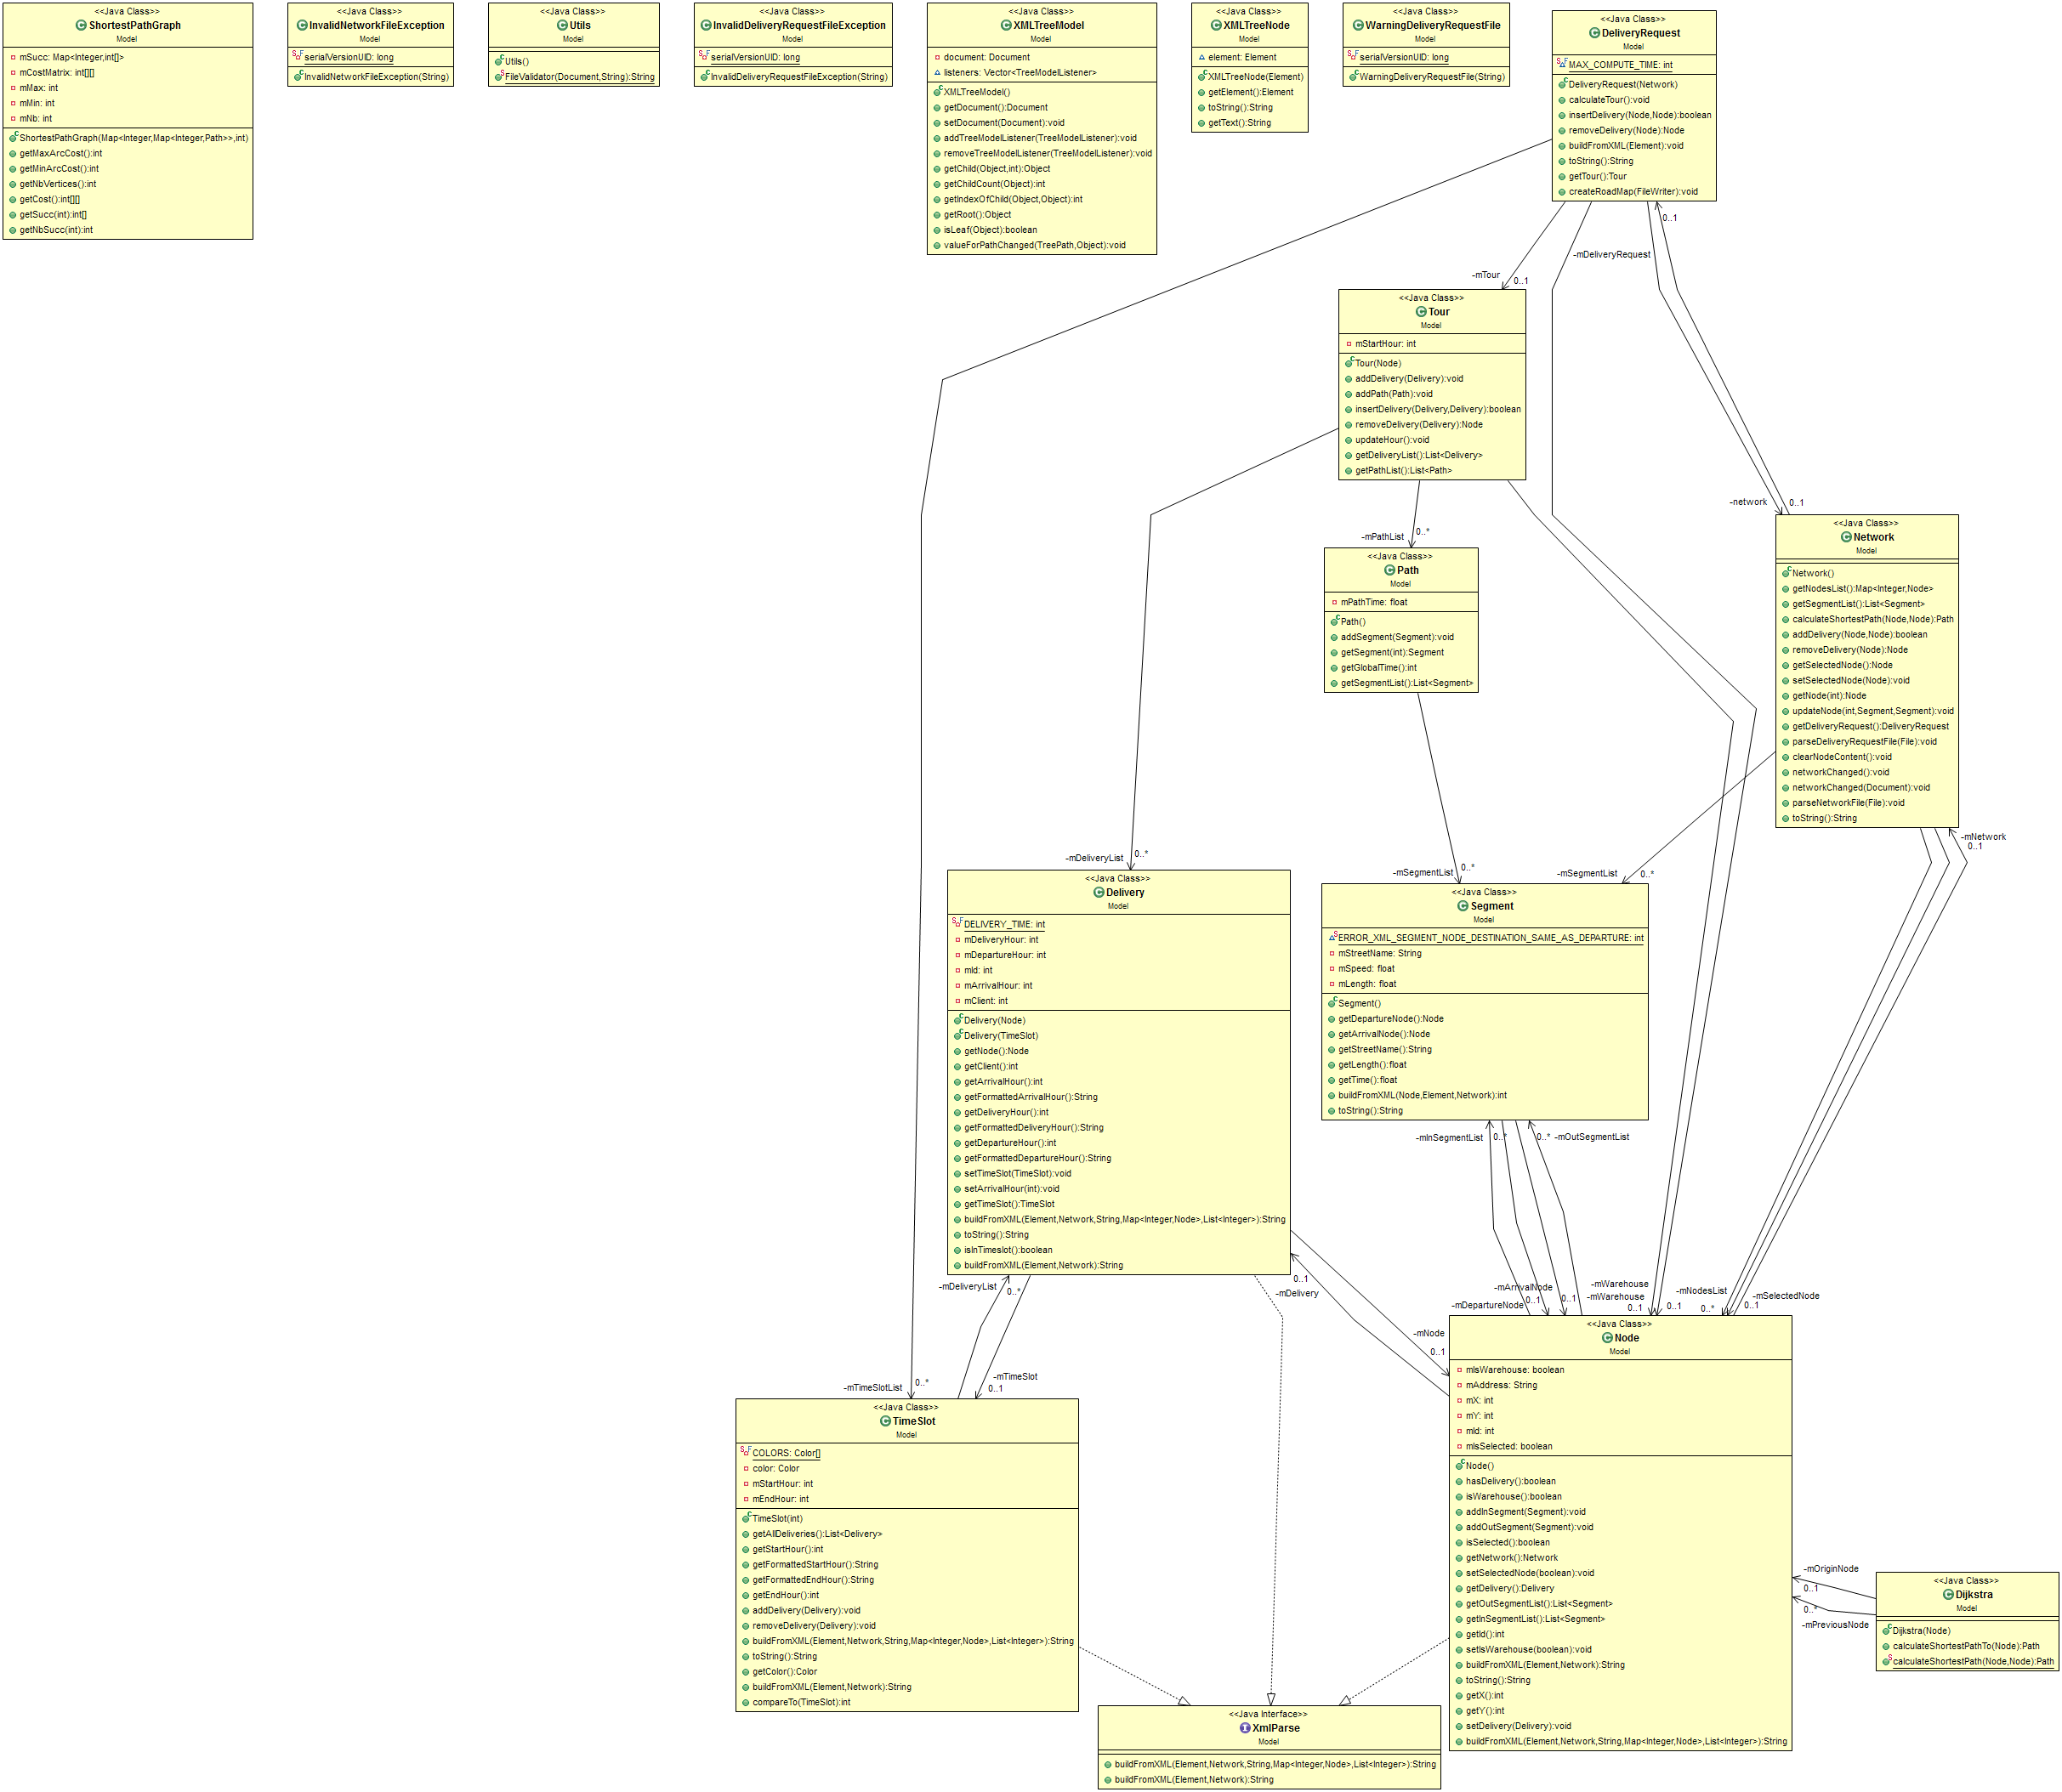
\includegraphics[width=\textwidth,height=\textheight,keepaspectratio]{Figures/retro_model}
		\rule{35em}{0.5pt}
	\caption[Diagramme de classes du package model]{Diagramme de classes du package model}
\end{figure}
\subsubsection{Dépendances}
\begin{figure}[H]
	\centering
		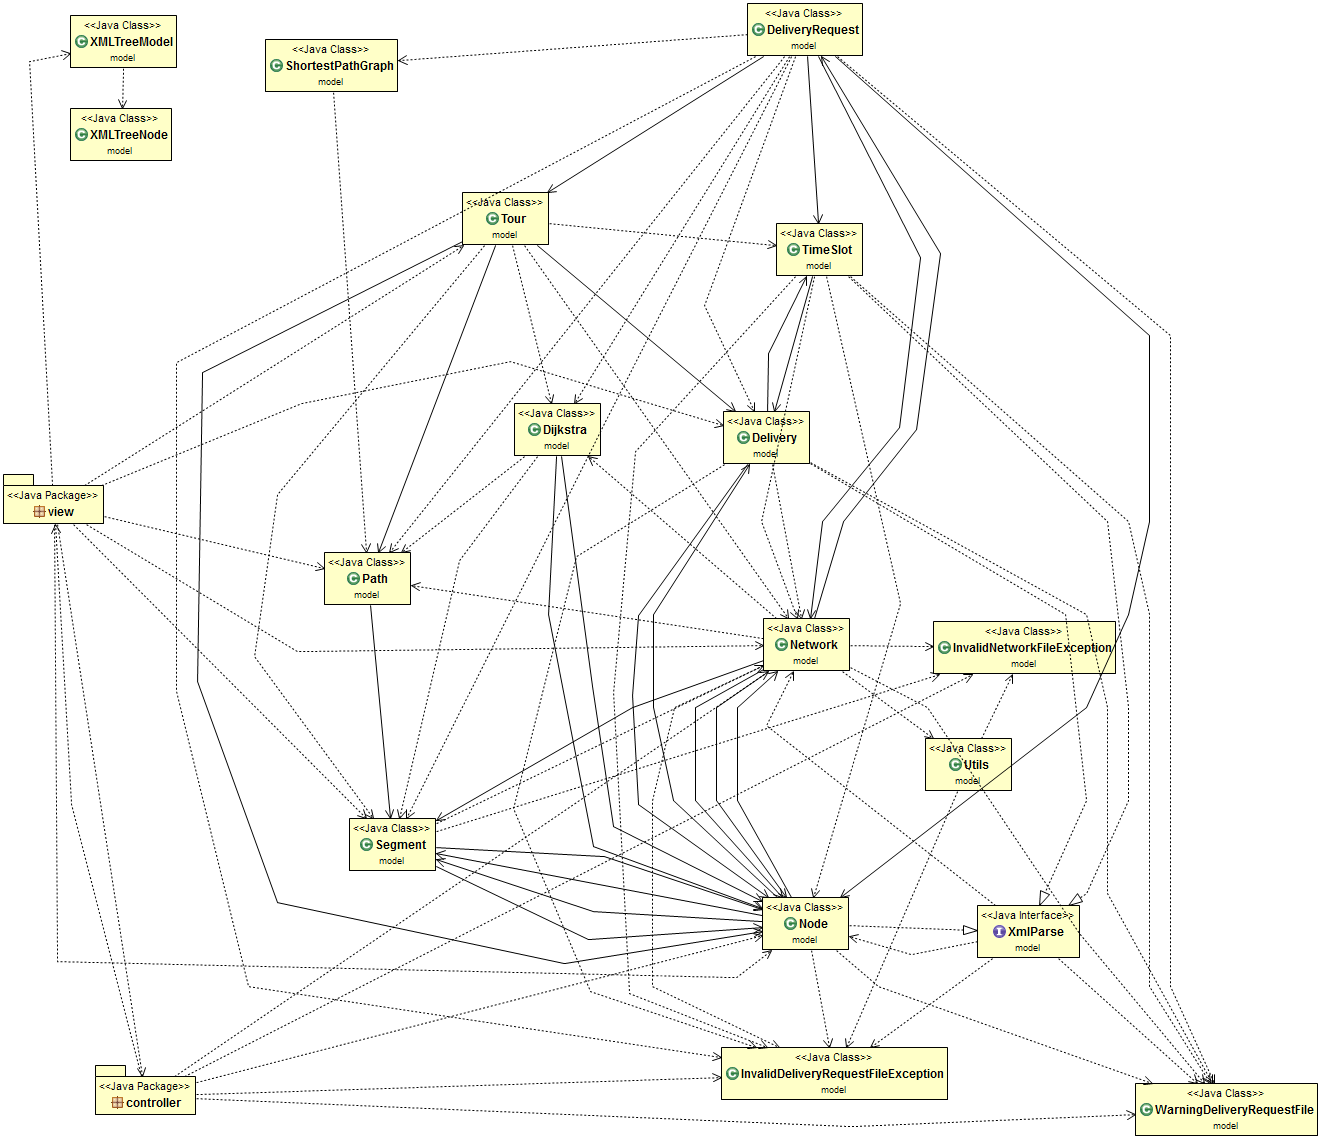
\includegraphics[width=\textwidth,height=\textheight,keepaspectratio]{Figures/retro_model_dep}
		\rule{35em}{0.5pt}
	\caption[Dépendances du package model]{Dépendances du package model}
\end{figure}
\subsubsection{Évolutions lors de l'implémentation}
Nous nous sommes globalement tenus à la conception initiale qui consistait à parser les fichiers XML de façon granulaire et descendante. Les changements intervenus sont dus à la gestion des Erreurs rédhibitoires et des “Warning”. 
L’idée de départ qui consistait à remonter des erreurs à chaque niveau de parse a été remplacé majoritairement par une validation du fichier XML grâce à un modèle xsd défini.
Le modèle xsd pour le réseau fournit les vérifications suivantes :
\begin{itemize} 
\item La bonne présence des balises, de leurs attributs et de l’exactitude de leur type (définition d’un type utilisateur vérifiant la syntaxe des vitesses et longueurs).
\item L’unicité des id des noeuds du réseau
\item Le noeud destination d’un tronçon sortant appartient bien au réseau (contrainte de clé référentielle).
\end{itemize}
Le modèle xsd pour les livraisons fournit les vérifications suivantes : 
\begin{itemize}
\item La bonne présence des balises, de leurs attributs et de l’exactitude de leur type (définition d’un type utilisateur vérifiant la syntaxe des heures de début et de fin des plages horaires).
\item L’unicité de l’Entrepot.
\end{itemize}
Certaines vérifications se font néanmoins dans le code et sont gérés par le principe de levée d’Exception (Erreurs et Warning). Principalement pour les erreurs rédhibitoires : la gestion des noeuds “impasses” et “ilots”, les livraisons sur des noeuds inexistants dans le réseau chargé, les heures incohérentes pour les plages de livraison. Et pour les “warning” : client avec plusieurs adresses, plages horaires vides...
Cette gestion en Erreurs et Warning n’ayant pas été pensé en amont, cela nous a posé quelques problèmes dus à des oublis ou maladresses lors de l'implementation..

En ce qui concerne le calcule d'une tournée, suite à l’implémentation des classes et des diagrammes de séquences relatifs aux calculs de la tournée, nous avons identifié plusieurs points d’évolution. Ces modifications ont été effectuées pour plusieurs raisons.
Dans un premier temps, nous avons éludé le calcul des plus courts chemins (Dijkstra) en supposant que l’algorithme serait effectué uniquement en une méthode de la classe Network sans accès aux classes extérieures. En réalité, cette opération ne necessite que le noeud de départ, les autres informations étant extraites de ses attributs. Nous avons donc déplacer ce calcul et créer une classe dédiée. De plus, cette classe permet de stocker des résultats temporaires et d’accélerer les calculs.

\subsection{Package view}
\subsubsection{Diagramme de classes rétro-générés}
\begin{figure}[H]
	\centering
		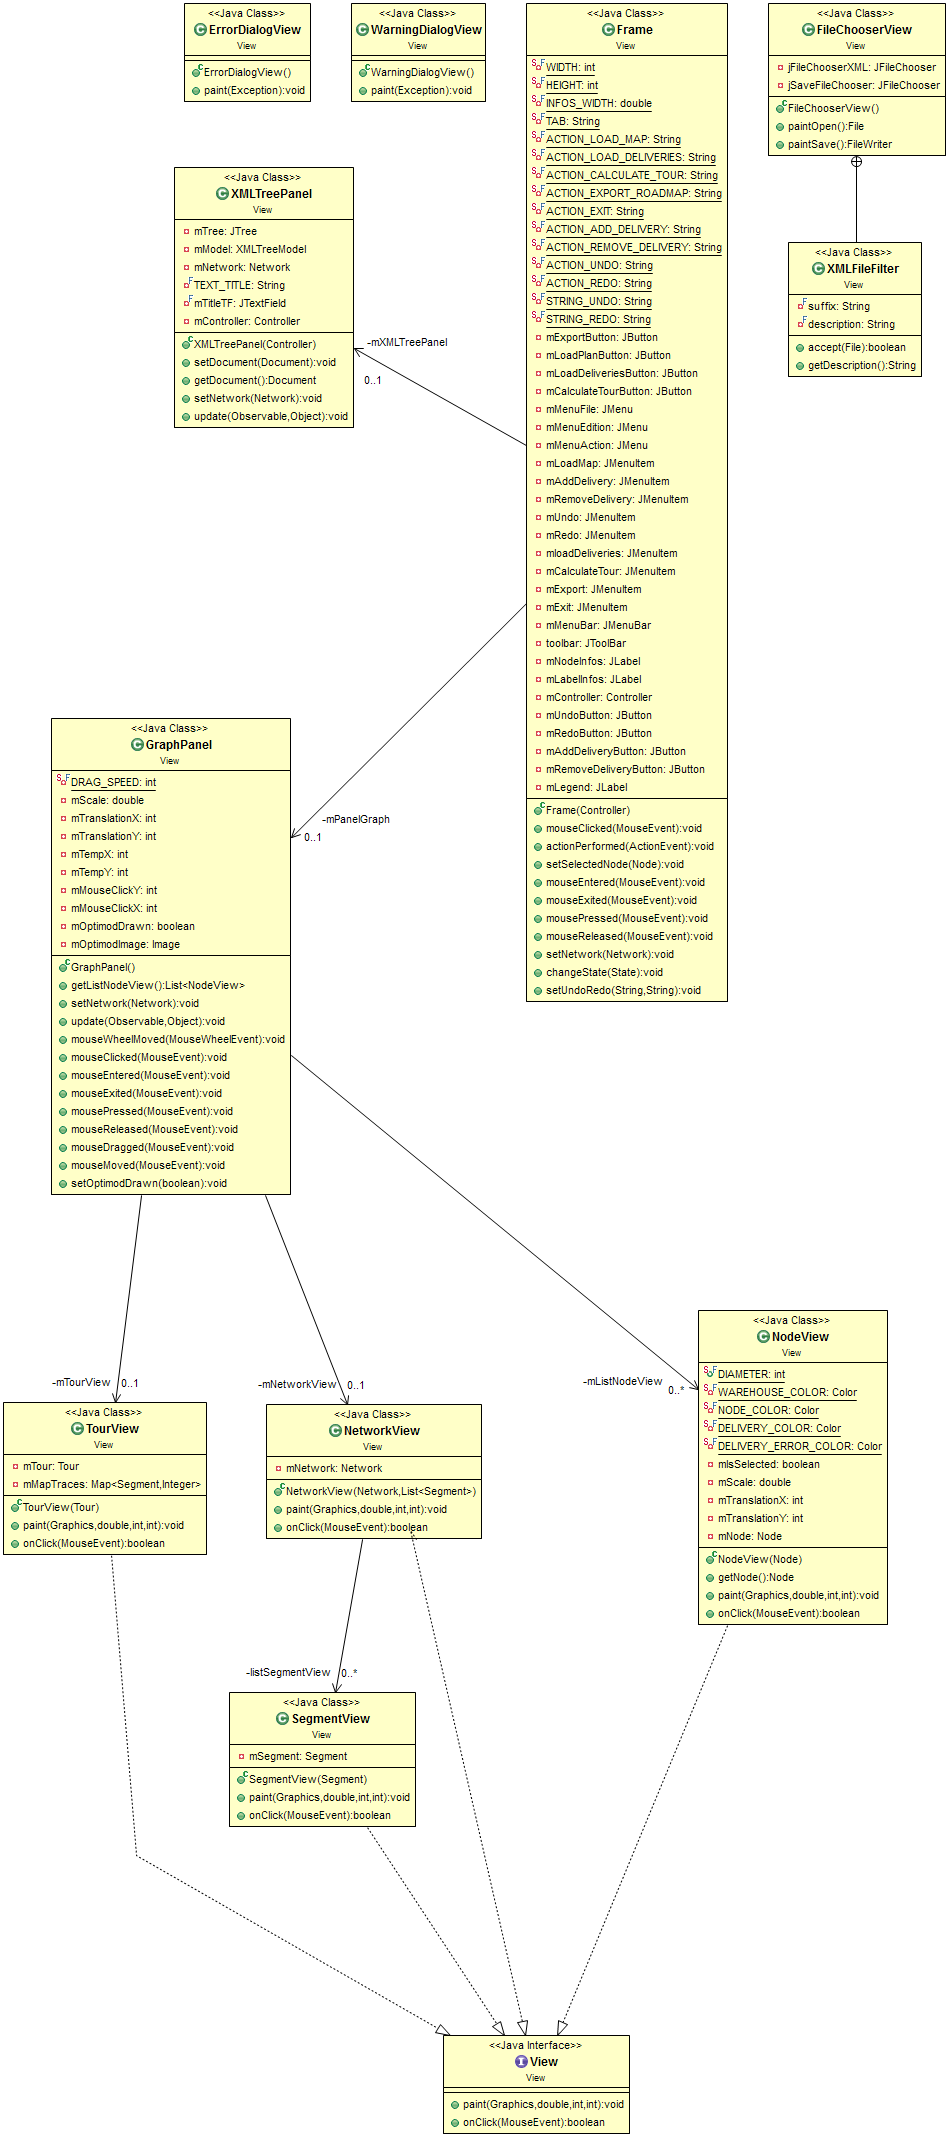
\includegraphics[width=\textwidth,height=\textheight,keepaspectratio]{Figures/retro_view}
		\rule{35em}{0.5pt}
	\caption[Diagramme de classes du package view]{Diagramme de classes du package view}
\end{figure}
\subsubsection{Dépendances}

\begin{figure}[H]
	\centering
		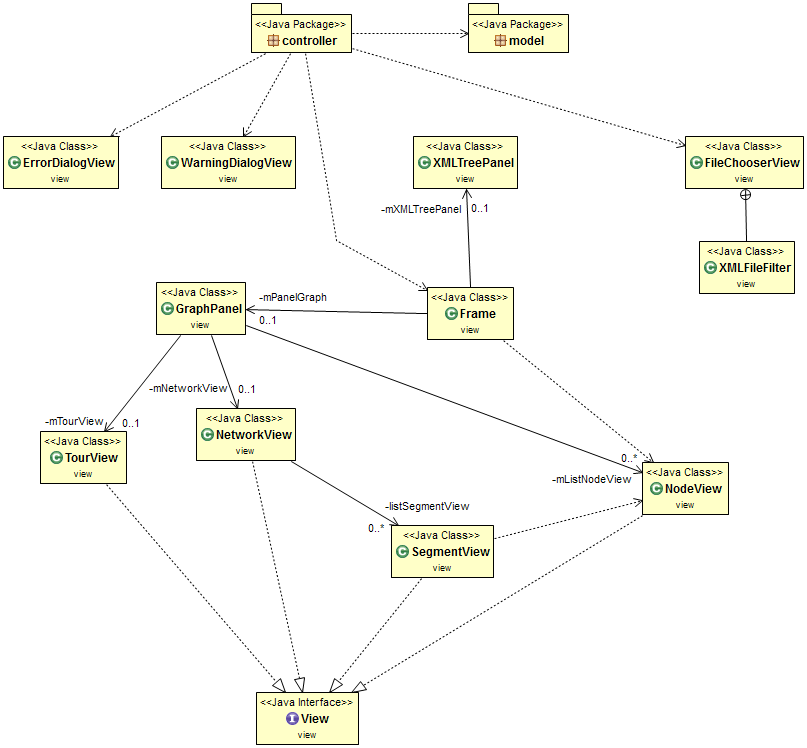
\includegraphics[width=\textwidth,height=\textheight,keepaspectratio]{Figures/retro_view_dep}
		\rule{35em}{0.5pt}
	\caption[Dépendances du package view]{Dépendances du package view}
\end{figure}

\subsubsection{Évolutions lors de l'implémentation}
Nous avons du revenir sur nos choix faits lors de la création des diagrammes de séquence pour l’ajout d’une livraison. Certains changements sont du au fait que nous avons finalement décidé d’implémenter le design pattern State pour une meilleure gestion des boutons à activer dans la fenêtre. Nous avons aussi décidé de rajouter une classe Invoker pour que la gestion des piles de commandes soit séparée du controleur. Nous avons aussi décidé d’ajouter un attribut selectedNode au Network pour éviter d’avoir à parcourir trop souvent la liste des noeuds du 
réseaux pour trouver celui qui est sélectionné. Un autre point important auquel nous n’avions pas pensé lors de la conception est l’ajout où le suppression de livraisons avec l’entrepôt juste avant ou après. En effet, l’entrepôt n’étant pas dans la liste des livraisons, il s’agit d’un cas particulier. Enfin nous avons modifié la méthode onClick pour qu’elle se contente d’indiquer si le noeud est sélectionné ou non car nous avons pensé qu’il était plus propre de lancer le reste du traitement à partir de la Frame.

\subsection{Package controller}
\subsubsection{Diagramme de classes rétro-générés}
\begin{figure}[H]
	\centering
		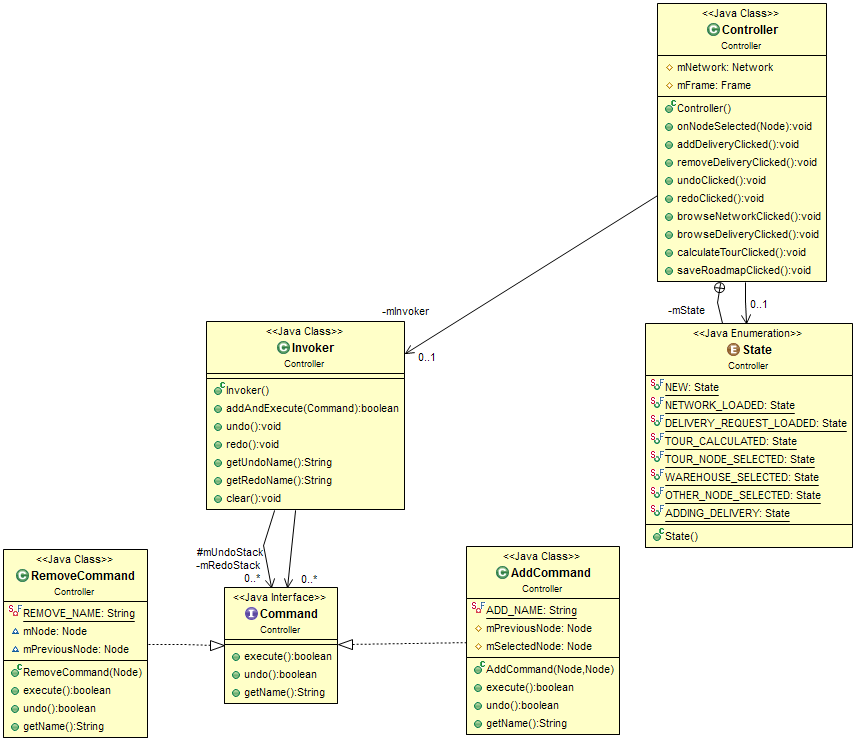
\includegraphics[width=\textwidth,height=\textheight,keepaspectratio]{Figures/retro_controller}
		\rule{35em}{0.5pt}
	\caption[Diagramme de classes du package controller]{Diagramme de classes du package controller}
\end{figure}
\subsubsection{Dépendances}

\begin{figure}[H]
	\centering
		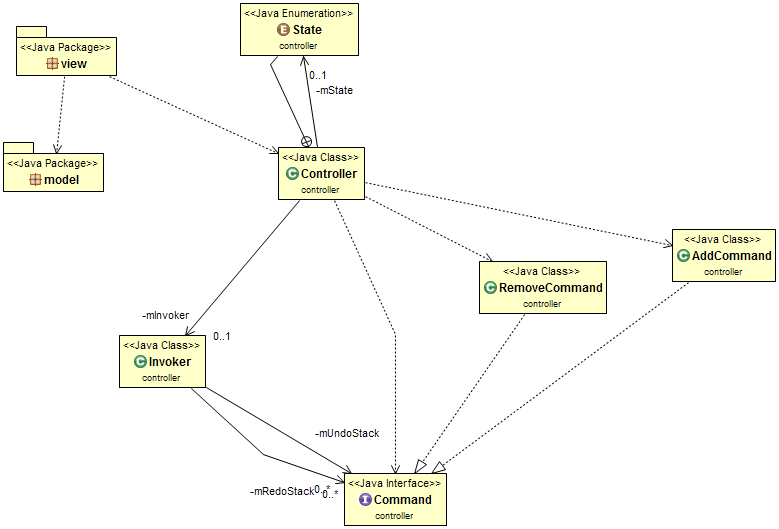
\includegraphics[width=\textwidth,height=\textheight,keepaspectratio]{Figures/retro_controller_dep}
		\rule{35em}{0.5pt}
	\caption[Dépendances du package controller]{Dépendances du package controller}
\end{figure}
\subsubsection{Évolutions lors de l'implémentation}
Nous avons décidé de créer une classe dédiée à la gestion des opérations (Annuler / Refaire). En effet, ces opérations étaient précedemment effectuées dans le controller. Pour mieux respecter le “Design Pattern Command” et devant la complexité de cette classe, nous avons choisi de déplacer certaines opérations dans un Invoker.


%----------------------------------------------------------------------------------------
%	SECTION 2
%----------------------------------------------------------------------------------------

\section{Captures d'écran de l'application}
\begin{figure}[H]
	\centering
		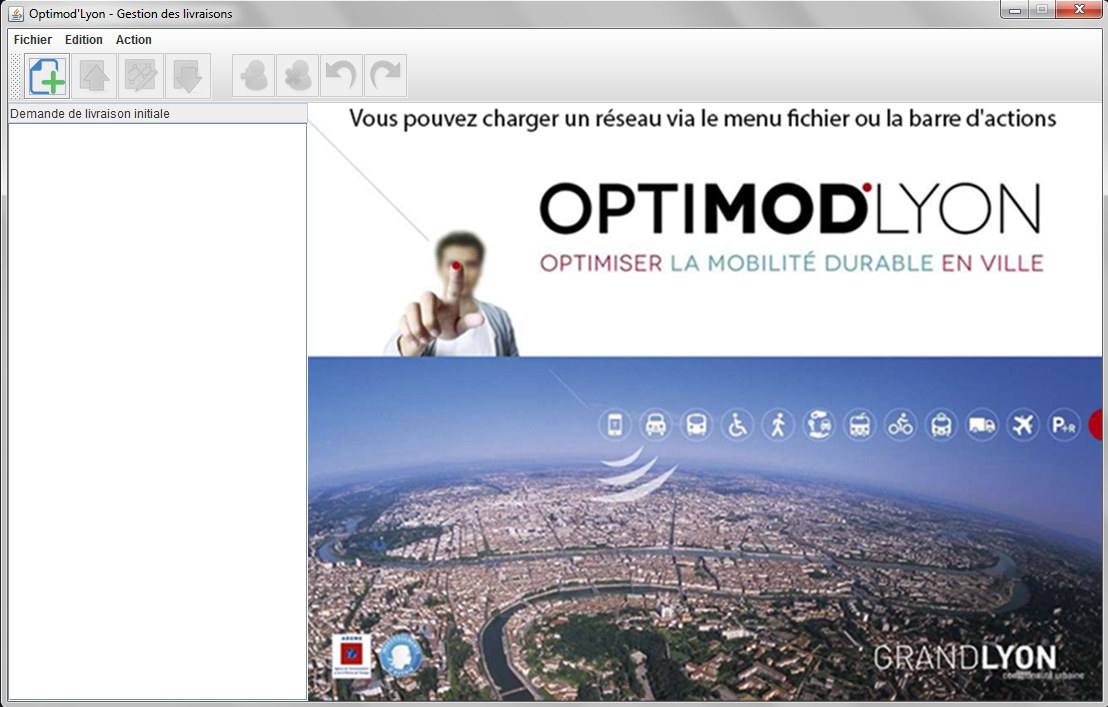
\includegraphics{Figures/welcome}[width=\textwidth,height=\textheight,keepaspectratio]
		\rule{35em}{0.5pt}
	\caption[Fenêtre d'accueil de l'application]{Fenêtre d'accueil de l'application}
\end{figure}
\begin{figure}[H]
	\centering
		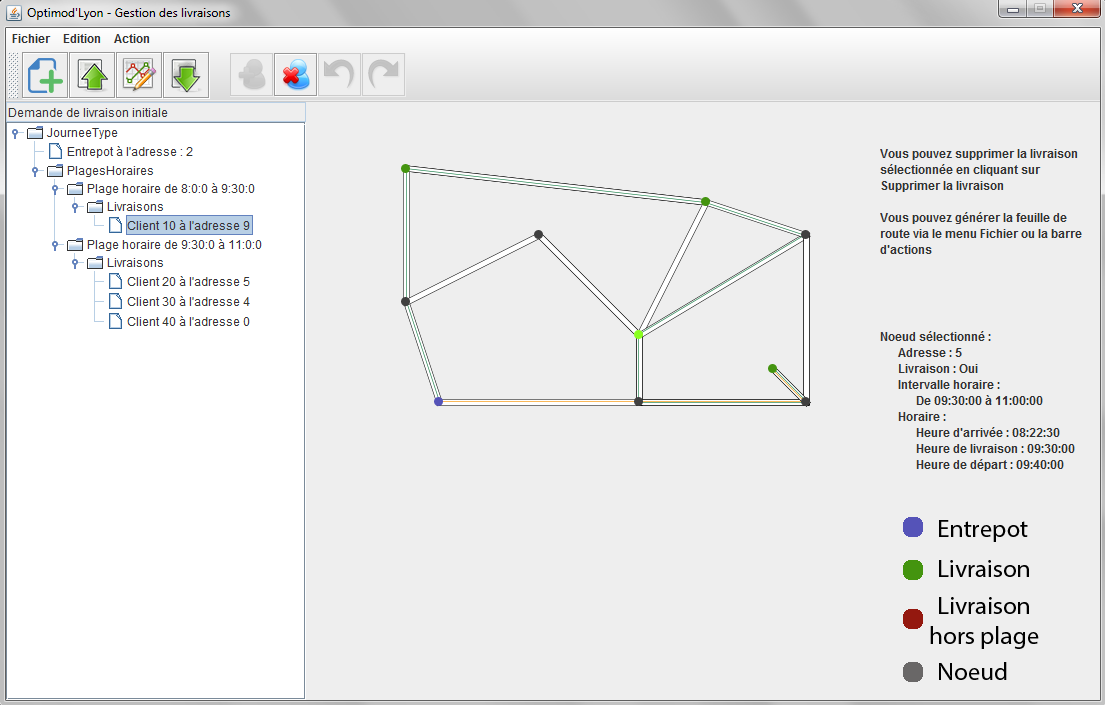
\includegraphics{Figures/plan}[width=\textwidth,height=\textheight,keepaspectratio]
		\rule{35em}{0.5pt}
	\caption[Visualisation du plan d'une zone géographique]{Visualisation du plan d'une zone géographique}
\end{figure}
\begin{figure}[H]
	\centering
		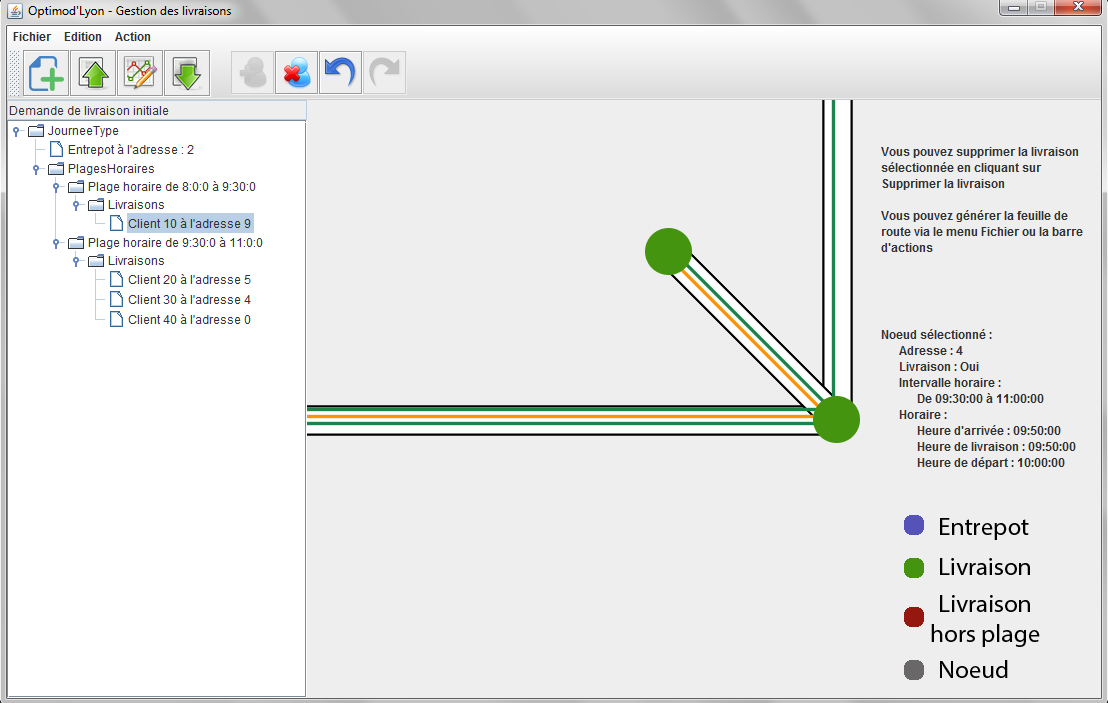
\includegraphics{Figures/path}[width=\textwidth,height=\textheight,keepaspectratio]
		\rule{35em}{0.5pt}
	\caption[Superposition d'itinéraires]{Superposition d'itinéraires}
\end{figure}